\chapter{Основы построения запросов}
\section{Основы языка T-SQL}

Язык Transact-SQL (T-SQL) --- это основной язык, используемый для управления данными и их обработки в Microsoft SQL Server. T-SQL — это диалект стандартного языка SQL.

\begin{figure}[h!]
	\begin{center}
		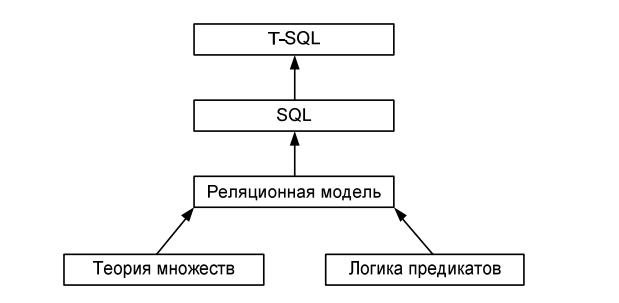
\includegraphics[width=0.8\textwidth]{img/tsql.png}
	\end{center}
	\captionsetup{justification=centering}
	\caption{Эволюция языка T-SQL}
	\label{img:ev}
\end{figure}

Следование стандарту при написании кода считается наилучшим решением. Это
делает код более переносимым. Если диалект, на котором вы пишете, поддерживает и стандартный, и нестандартный способы выполнения каких-либо операций, всегда следует выбирать стандартный способ. Нестандартный режим стоит выбирать только в том случае, если он
дает заметное преимущество, не предоставляемое стандартным режимом. 

Основой стандартного языка SQL является \textit{реляционная модель}, представляющая собой математическую модель для управления и обработки данных. Отношение в реляционной модели — это то, что в SQL называется таблицей.

SQL пытается представить отношение с помощью
таблицы: отношение имеет заголовок и тело. Заголовок — это набор атрибутов (которые SQL пытается представить в виде столбцов), каждый определенного типа.
Атрибут определяется именем и именем типа. Тело отношения представляет собой
множество кортежей (которые SQL пытается представить в виде строк). Каждый
заголовок кортежа — это заголовок отношения. Каждое значение атрибута кортежа
имеет соответствующий тип.

\begin{figure}[h!]
	\begin{center}
		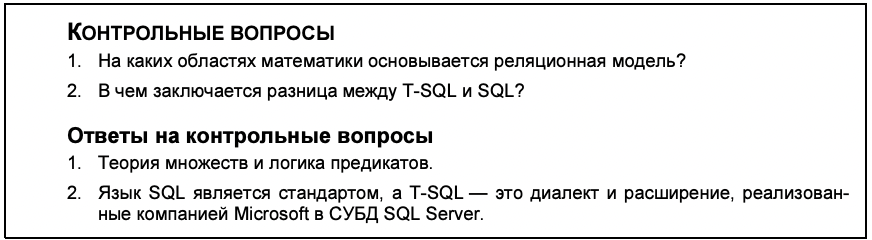
\includegraphics[width=0.8\textwidth]{img/control1.png}
	\end{center}
	\captionsetup{justification=centering}
\end{figure}


Вот пример неправильной терминологии в T-SQL. Термины <<поле>> (field) и <<запись>> (record) для обозначения того, что в T-SQL называется <<столбец>> (column) и
<<строка>> (row) соответственно. Поля и записи — это физические понятия. Поля —
это то, что отображается в пользовательском интерфейсе в клиентских приложениях, а записи — это то, что имеется в файлах и курсорах. Таблицы являются логическими структурами и имеют логические строки и столбцы.
Еще один пример неверной терминологии связан с <<NULL-величинами>>. NULL — это
обозначение отсутствующего значения, а не собственно величины. Поэтому правильное использование этого термина — <<NULL-маркер>> или просто NULL. 

\begin{figure}[h!]
	\begin{center}
		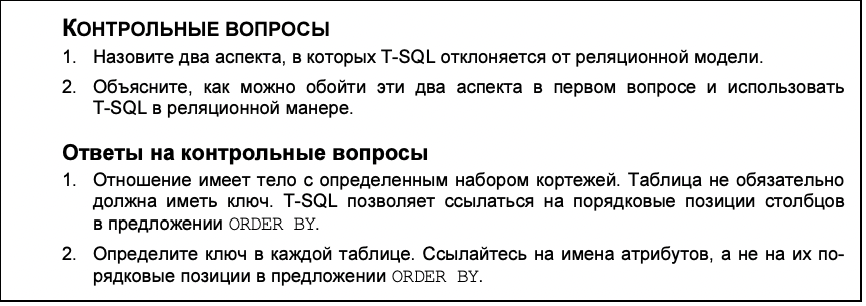
\includegraphics[width=0.7\textwidth]{img/control2.png}
	\end{center}
	\captionsetup{justification=centering}
\end{figure}

\begin{figure}[h!]
	\begin{center}
		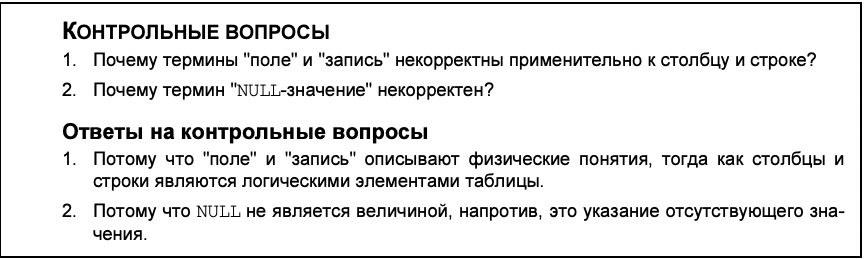
\includegraphics[width=0.7\textwidth]{img/control3.png}
	\end{center}
	\captionsetup{justification=centering}
\end{figure}


\subsection*{Резюме занятия}
\begin{itemize}
	\item Язык T-SQL имеет строгие математические основы. Он основывается на стандартном SQL, который, в свою очередь, основывается на реляционной модели,
	в свою очередь основывающейся на теории множеств и логике предикатов.
	\item Важно понимать принципы реляционной модели и применять их при написании
	кода T-SQL. 
	\item При описании концепций в T-SQL необходимо использовать правильную терминологию, поскольку это влияет на ваши знания. 
\end{itemize}

\subsection*{Закрепление материала}

\begin{figure}[h!]
	\begin{center}
		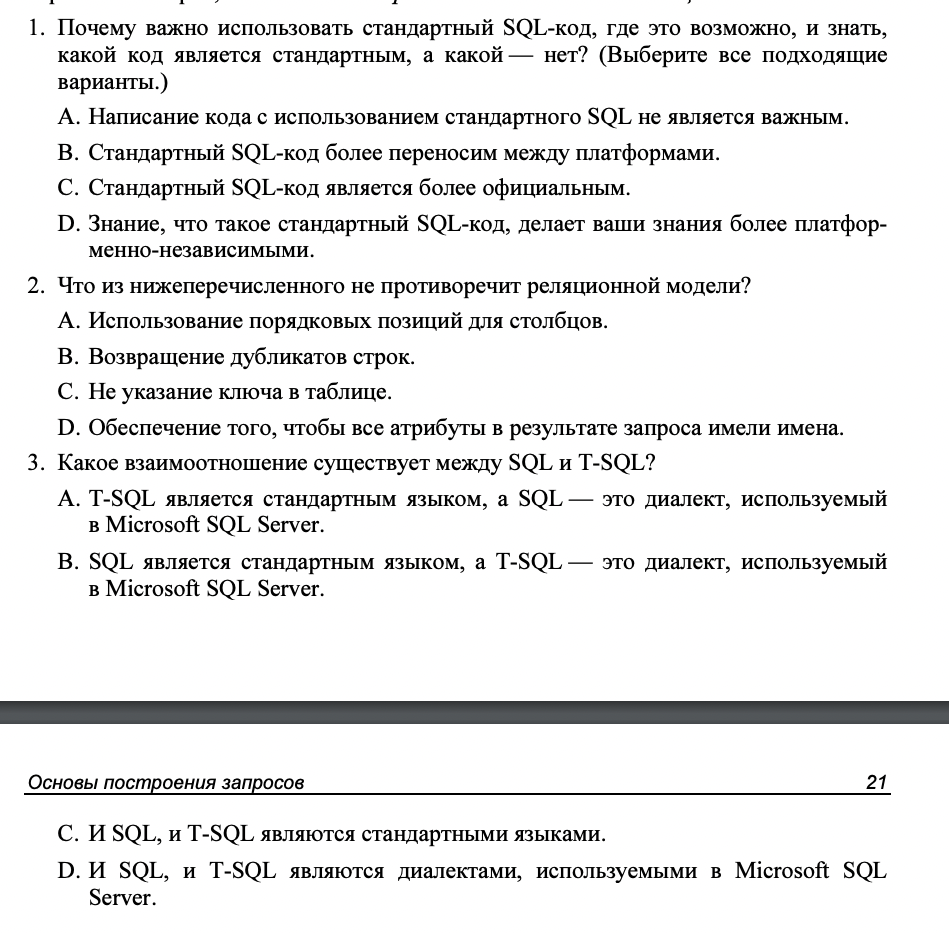
\includegraphics[width=0.7\textwidth]{img/zakrep1.png}
	\end{center}
	\captionsetup{justification=centering}
\end{figure}

\subsection*{Ответы}

\begin{figure}[h!]
	\begin{center}
		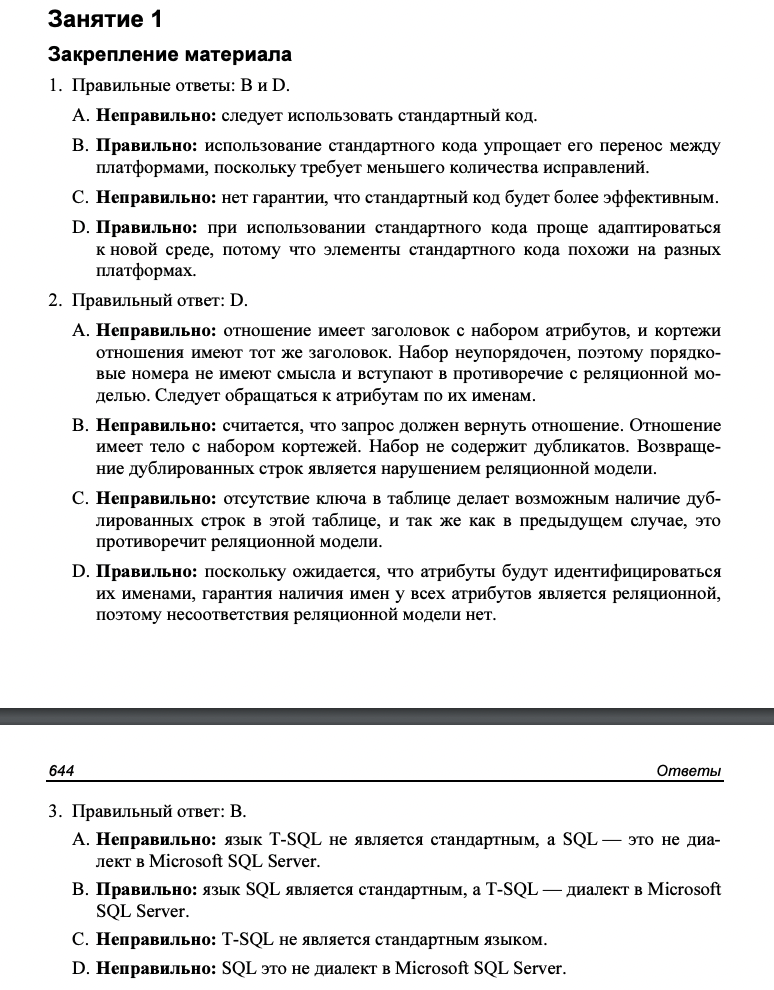
\includegraphics[width=0.7\textwidth]{img/ans1.png}
	\end{center}
	\captionsetup{justification=centering}
\end{figure}




\section{Понимание логической обработки запросов}
У языка T-SQL имеется как физическая, так и логическая сторона. Логическая сторона — это концептуальная интерпретация запроса, которая объясняет, что является корректным результатом запроса. Физическая сторона — это обработка запроса
ядром базы данных (компонентом Database Engine). Физическая обработка должна
дать результат, определенный логической обработкой запроса. Для достижения
этой цели ядро базы данных может использовать оптимизацию. Оптимизация
способна изменить последовательность шагов логической обработки запроса или
удалить их вовсе, но только при условии, что результат остается тем, который
определен логической обработкой запроса.

Логическая последовательность обработки запросов шести основных предложений запросов: 

\begin{enumerate}
	\item FROM.
	\item WHERE.
	\item GROUP BY.
	\item HAVING.
	\item SELECT.
	\item ORDER BY.
\end{enumerate}

\begin{figure}[h!]
	\begin{center}
		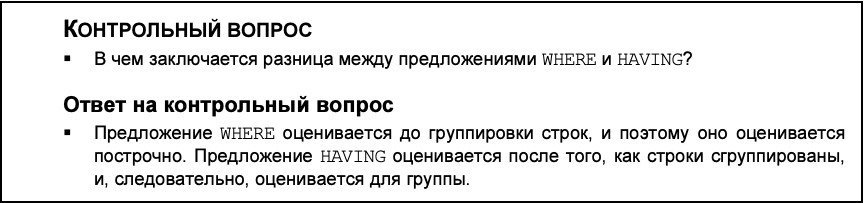
\includegraphics[width=0.9\textwidth]{img/control4.png}
	\end{center}
	\captionsetup{justification=centering}
\end{figure}

\begin{figure}[h!]
	\begin{center}
		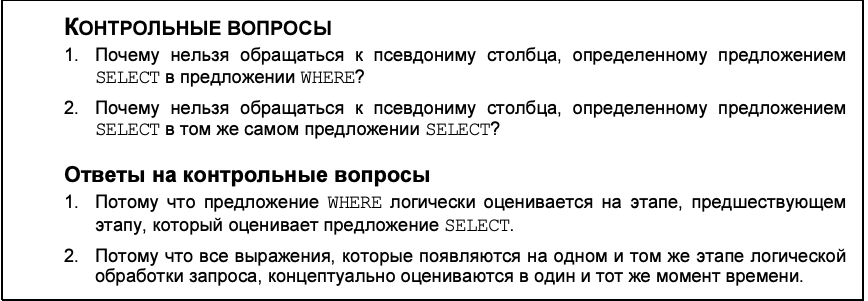
\includegraphics[width=0.9\textwidth]{img/control5.png}
	\end{center}
	\captionsetup{justification=centering}
\end{figure}

\subsection*{Резюме занятия}
\begin{itemize}
	\item Язык T-SQL разработан как декларативный язык, в котором инструкции представлены в англо-подобном виде. Таким образом, подобный вводу с клавиатуры порядок предложений в запросе начинается с предложения \textit{SELECT}. 
	\item Логическая обработка запросов является концептуальной интерпретацией запроса, определяющей корректный результат, и в отличие от подобного вводу с клавиатуры порядка предложений в запросе, она начинается с оценивания предложения \textit{FROM}. 
\end{itemize}


\subsection*{Закрепление материала}

\begin{figure}[h!]
	\begin{center}
		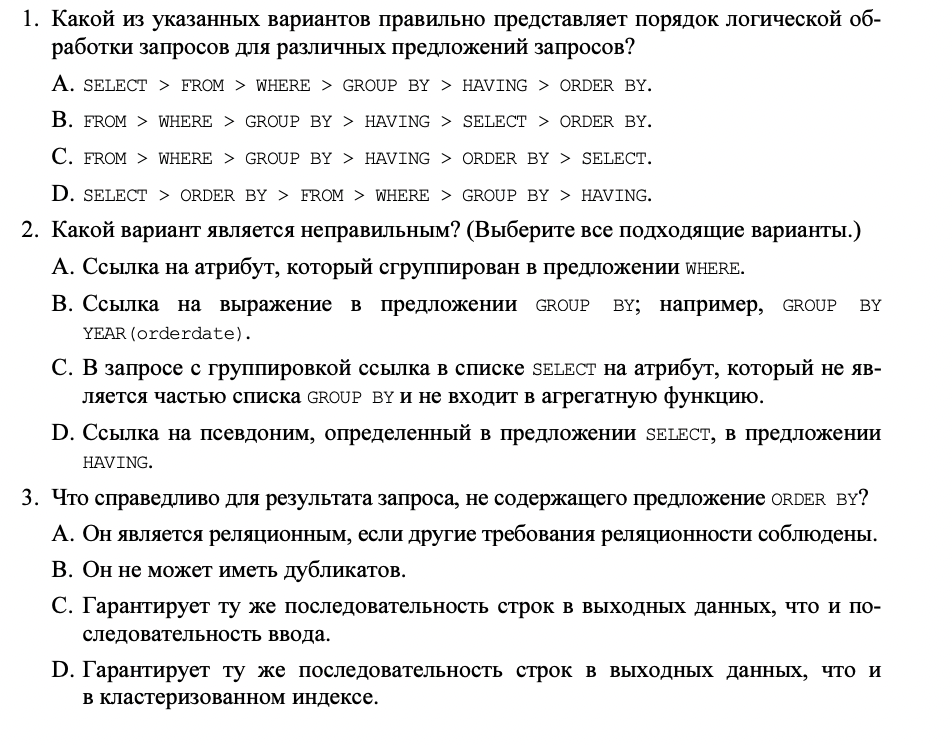
\includegraphics[width=0.9\textwidth]{img/zakrep2.png}
	\end{center}
	\captionsetup{justification=centering}
\end{figure}

\subsection*{Ответы}

\begin{figure}[h!]
	\begin{center}
		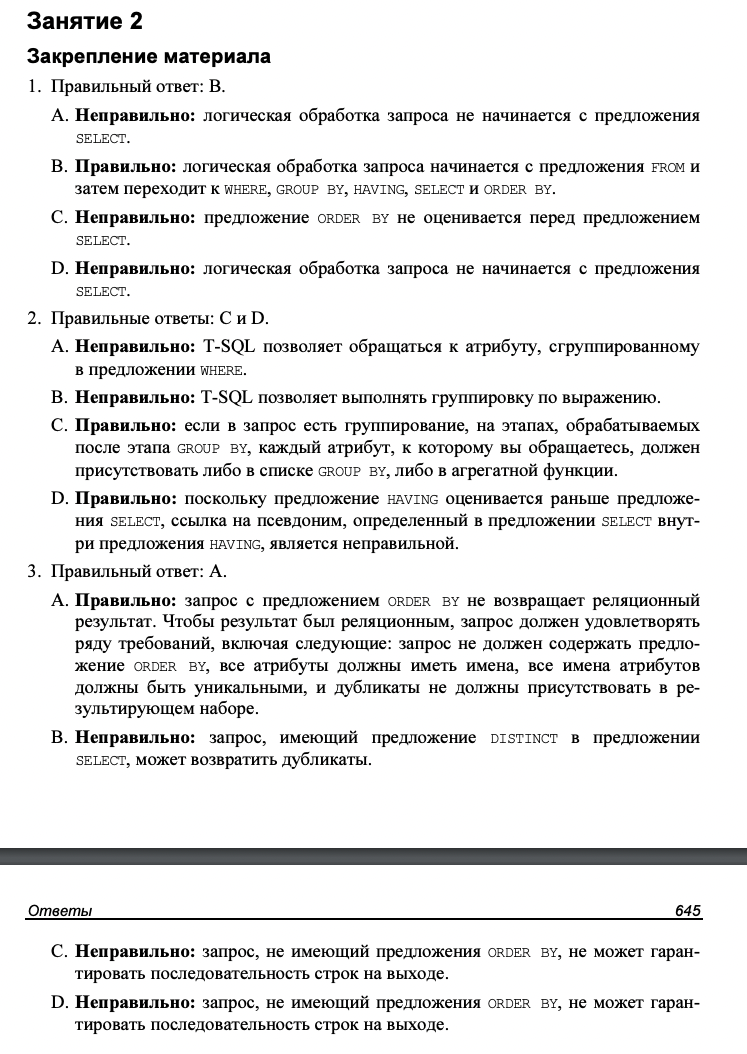
\includegraphics[width=0.7\textwidth]{img/ans2.png}
	\end{center}
	\captionsetup{justification=centering}
\end{figure}

\newpage
\subsection*{Упражнения}

\begin{figure}[h!]
	\begin{center}
		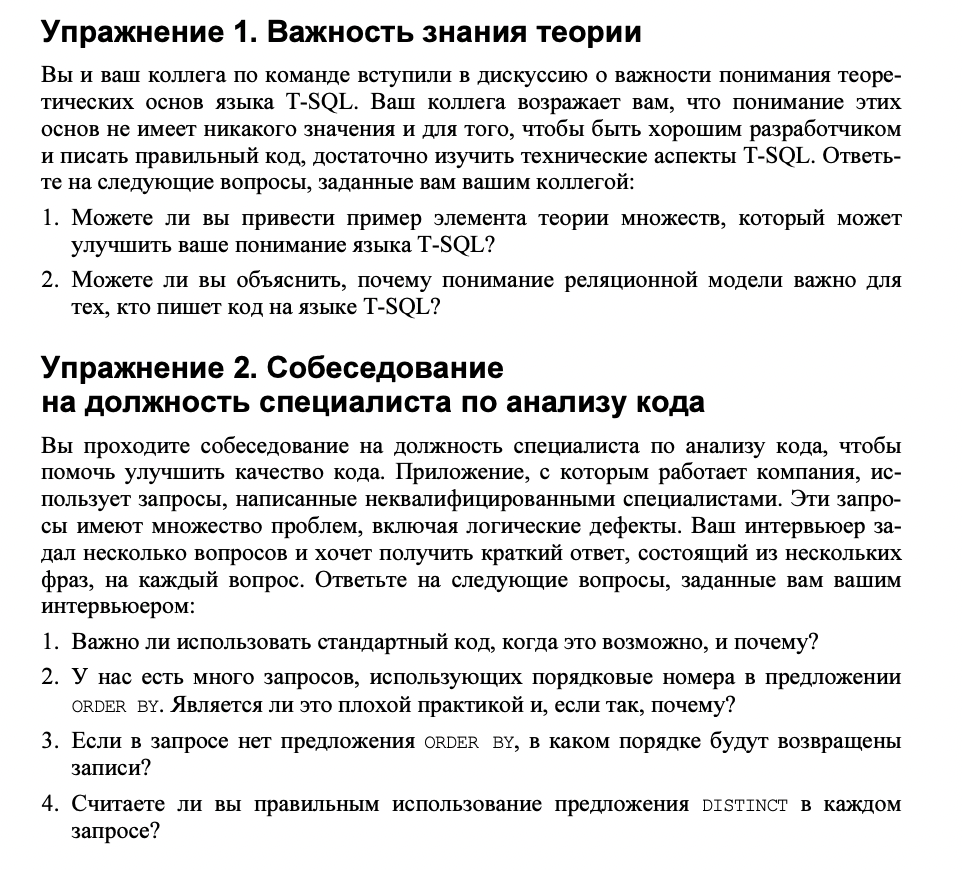
\includegraphics[width=0.9\textwidth]{img/ex1.png}
	\end{center}
	\captionsetup{justification=centering}
\end{figure}

\subsection*{Ответы}

\begin{figure}[h!]
	\begin{center}
		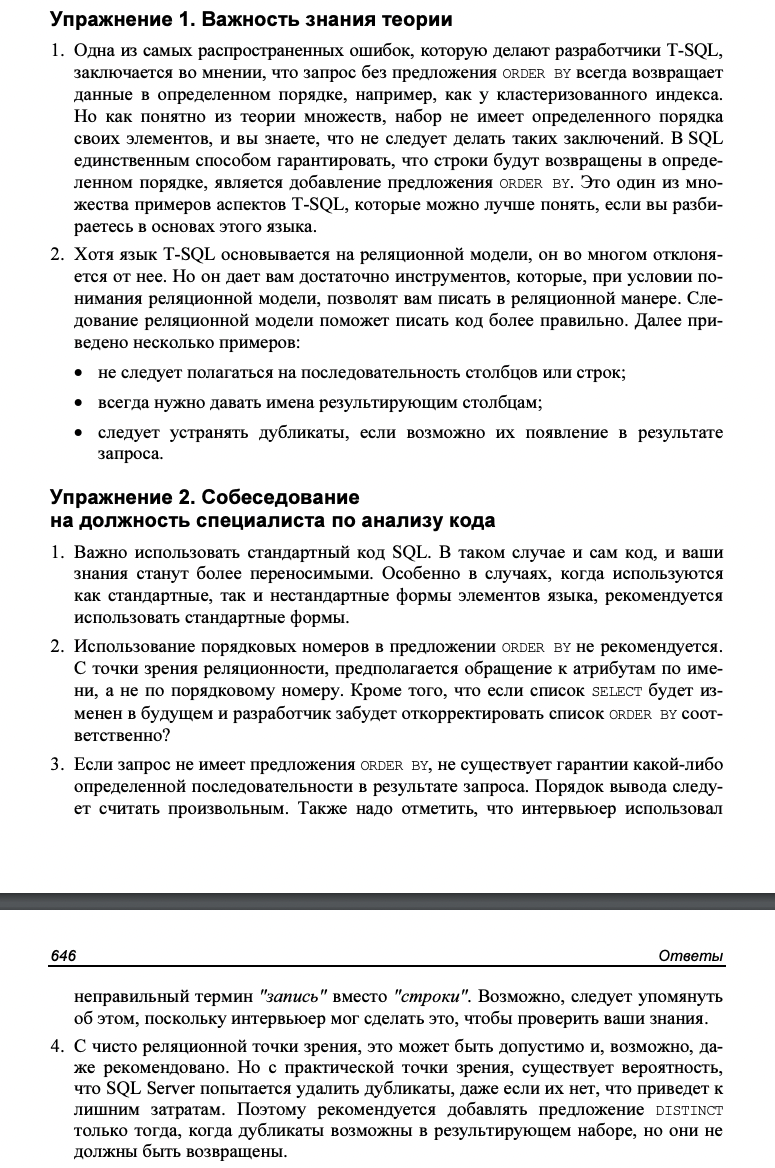
\includegraphics[width=0.9\textwidth]{img/eans1.png}
	\end{center}
	\captionsetup{justification=centering}
\end{figure}